\section{Parallelization}
\label{sec:parallelization}

\subsection{Loop Dependencies} 
\label{sec:loopdependencies}

Array loop optimization is a crucial component of compiler design. More specifically
the optimizations that can be done on arrays \emph{within} a loop make better use of 
parallelization which results in decreased running times. The effectiveness of the 
optimization is entirely dependent on two factors: the number of processing threads
available, and the dependencies between the statements of the loop. These dependencies 
come in two types: Control-dependencies and data-dependencies. Control dependencies
exist between statements where the control flow of the program determines
program execution. Data-dependencies are dependencies that exist 
between nodes based on their interaction with shared data.

Aiken et al. \cite{Aiken1988} provides an illustration of data-dependencies. 
Consider the code in \figref{fig:arrayloop}. Line 2 is not dependent on any other 
line calculated in the same iteration. Line 5 is dependent on the calculation 
of lines 3, and 4. More interestingly lines 3, 4 are not only dependent on line 2, 
but also on a \emph{previous calculation} of line 5. 

\begin{figure}[h]
\centering
\begin{minipage}{0.70\textwidth}
\begin{javacode}
	for(int i = 0; i < N; i++) {
		A[i] = B[i];
		B[i] = A[i] * D[i - 1];
		C[i] = A[i] * D[i - 1];
		D[i] = B[i] * C[i]; 
	}
\end{javacode}
\end{minipage}
\caption{Loop containing array dependencies, a modified example from Aiken et al. \cite{Aiken1988}.}
\label{fig:arrayloop}
\end{figure}

\begin{figure}[h]
\centering
\begin{minipage}{0.70\textwidth}
\begin{javacode}
  if(<Cond1>) {
      <Stmt1>
  } else if(<Cond2>) {
      <Stmt2>
  } else {
      <Stmt3>
  }
\end{javacode}
\end{minipage}
\caption{If-Then-Else dependency.}
\label{fig:ifthenelsedep}
\end{figure}


Every data-dependency either effects variables within the current loop iteration
(intra-loop dependency) or effects variables on a different loop iteration
(across-loop dependency). One type of simple across-loop dependency occurs when a single
variable is modified by a previous calculation of itself. This is a trivial case,
but still counts as an across-loop dependency. Data dependences are preserved in the 
transformation to target MPC code. 


The most common type of control-dependency is the If-Then-Else dependency shown
in \figref{fig:ifthenelsedep}. The execution of each statement is dependent on the various conditionals 
present. In this example all three statements are dependent on the outer if conditional while only
statements 2 and 3 are dependent on inner conditional. Control dependences 
are ``inverted'' in the target MPC code. Instead of dependencies between the branch statements
to the conditional, there will be a dependence from statement 2 and 3 to the MUX 
node, as well as a dependecy between the MUX node and the conditional. 

\subsection{HPC Parallelization}
\label{sec:hpcparallelization}

In the High performance computing (HPC) world a schedule is created to minimize the number
of sequential instructions of a program by utilizing a fixed number of threads. There 
are two main factors that determine the extent to which optimization can take place.
The first are control and data dependencies discussed above. The second is the number
of parallel processes that can be executed (i.e. the number of threads available). 
Importantly, each thread can perform arbitrary operations that are not reliant on the operations 
run on any other thread. The optimal schedule is then that which achieves the minimum number 
of sequential steps, while both preserving inter-loop and cross-loop dependencies 
and maximizing resource use. 
% In HPC optimizations \ana{Incomplete sentence?}.

Schedules are evaluated based off of their maximum \emph{delay}. The delay of a given 
schedule represents the number of steps between loop iterations that are 
carried out to preserve all looping dependencies \cite{Aiken1988}. 
For example, a variable modifying itself within a loop has a static distance of 1
iteration between the definition and usage. Creating a schedule with an optimal minimal delay
(steps between loop iterations) with a restricted number of processors has been shown to be
NP-hard \cite{Cytron1984},\cite{Graham1971},\cite{Darte2000}. 
Modern compilers often use heuristics to achieve a schedule
that is as close to optimal as possible. The classical HPC literature 
has considered different types of across-loop scheduling schemes. 
One scheduling scheme, called \emph{doacross}~\cite{Aiken1988},\cite{Cytron1986}, requires that all instructions in an 
iteration are scheduled on the same processor. 
The optimal doacross schedule for \figref{fig:arrayloop} (from \cite{Aiken1988}) is shown in \figref{fig:HPCexample} (b). 
Next, Aiken and Nicolau \cite{Aiken1988} proposed a new schedule, which they called
\emph{greedy} schedule, where instructions in an iteration can be scheduled on different processors. 
The optimal greedy schedule for our example, which achieves better minimal delay than the optimal 
doaccross schedule, is shown in \figref{fig:HPCexample}(c) (again, taken directly from~\cite{Aiken1988}). 

\begin{figure*}[tbhp]
\small
\begin{tabular}{lll}


\begin{minipage}[b]{4.20cm}
\centering
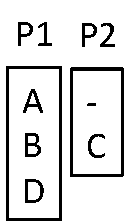
\includegraphics[width=0.4\textwidth]{images/HPCloop.pdf}
\end{minipage}

&

\begin{minipage}[b]{4.20cm}
\centering
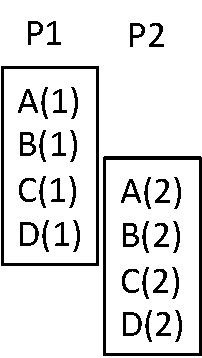
\includegraphics[width=0.4\textwidth]{images/HPCdoacrossLoop.pdf}
\end{minipage}

&

\begin{minipage}[b]{4.20cm}
\centering
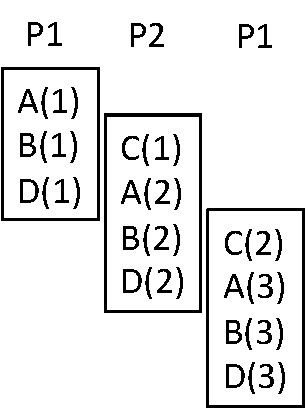
\includegraphics[width=0.6\textwidth]{images/HPCgreedyLoop.pdf}
\end{minipage}

\\

(a) Loop-body schedule
&
(b) Doacross across-loop schedule
& 
(c) Greedy across-loop schedule

\end{tabular}
\caption{Optimal HPC schedules. Different statements are each given letters. 
In (a) only one loop iteration is shown. In (b) and (c) variables 
are labeled according to both their statement (i.e A, B, C) and the loop iteration that is being 
computed which is shown in parentheses (A(1) represents the statement A on iteration 1).}
\label{fig:HPCexample}\vspace{-2ex}
\end{figure*}

\subsection{MPC Amortization}
\label{sec:mpcamortization} 

In MPC, the loop scheduling problem is different. Instead of having a fixed number of 
processors that carry out arbitrary independent operations, in MPC schedules the we assume that we can run
infinitely many operations (same operations) in parallel. We note that the relaxation of allowing infinite bandwidth 
is often made in the HPC setting as well and it is not necessarily valid in either case. 
Our current relies on this assumption however, in future work we plan to relax the 
assumption and extend our study and results.

%\lindsey{Ana, does something like this work? ``While there is still
%a practial limit to the number of operations that can be run in parallel it is not directly defined by the
%number of physical processors avaialable. We can also assume infinite processors in HPC, but this 
%fundamentally removes all constraits from the problem.'' This is to address wes's questions: We can do this in HPC waht is the diff}
%threads that can only run similar operations simultaneously.

For example, consider two separate operations A and B. We assume that both operations have 
the same constant running time. In classic HPC optimization both A and B can be run simultaneously with no 
restrictions as long as two processors are available to compute them. In MPC scheduling,
there is no restriction based on number of processors, but there is one on the types of
operations that are run in parallel. This means that there is only a benefit from amortization if A is run in parallel 
with another A operation, or B is run with another B operation. Our work aims to create a novel analysis 
that can be used to create schedules that improve the performance of MPC loops. 

% All similar operations  (in this case equality, 
% comparison, and subtraction) can be performed at the same cost as a single operation of that type. 

% \ana{Don't use the GCD example because it does not lend to parallelization. 
% Use the Aiken paper example, or the inner product example.}
% \figref{fig:gcdparallel}, shows a Java 8 examaple of how gcd() could be run in 
% parallel so each operation could benefit from amoritization. 

\begin{figure}[h]
\centering
\begin{minipage}{0.7\textwidth}
\begin{javacode}
  InnerProduct(A, B) {
      sum = 0;
      for(int i = 0; i < N; i++) {
          sum += A[i] * B[i];
      }
      return sum;
  }
\end{javacode}
\end{minipage}
\caption{Original inner product code.}
\label{fig:innerproduct}
\end{figure}

\begin{figure}[h]
\centering
\begin{minipage}{0.7\textwidth}
\begin{javacode}
  InnerProduct(A, B) {
      sum = 0
      for(int i = 0; i < N; i++) {
          tmp = MUL(A[i], B[i]);
          sum = ADD(sum, tmp);
      }
      return sum;
  }
\end{javacode}
\end{minipage}
\caption{MPC source for inner product.}
\label{fig:innerproductmpc}
\end{figure}

\begin{figure}[h]
\centering
\begin{minipage}{0.7\textwidth}
\begin{javacode}
  InnerProduct(A, B) {
      C = MUL(A, B, N)
      sum = 0
      for(int i = 0; i < N; i++) {
          sum = ADD(sum, C[i]);
      }
  }
\end{javacode}
\end{minipage}
\caption{Vectorized MPC source for inner product.}
\label{fig:innerproductmpcvec}
\end{figure}

\begin{figure}[h]
\centering
\begin{minipage}{0.7\textwidth}
\begin{javacode}
  int[][]  split_list(int[] A) {
      A = pad_array(A); // adds 0 to an odd length array
      int[][] B = new int[2][A.length / 2];
      for(int i = 0; i < A.length / 2; i++) {
          B[0][i] = A[2 * i];
          B[1][i] = A[(2 * i) + 1];
      }
      return B;
  }

  private static int  SUM(int[] A) {
      int[][] W = split_list(A);
      while(A.length > 1) {
          A = ADD_N(W[0], W[1]);
          W = split_list(A);
      }
      return A[0];
  }
  InnerProduct(A, B) {
      C = MUL(A, B, N)
      return SUM(C)
  }
\end{javacode}
\end{minipage}
\caption{Vectorized MPC source for inner product using divide and conquer.}
\label{fig:innerproductmpcvecdandc}
\end{figure}

\begin{figure}[h]
\centering
\begin{minipage}{0.7\textwidth}
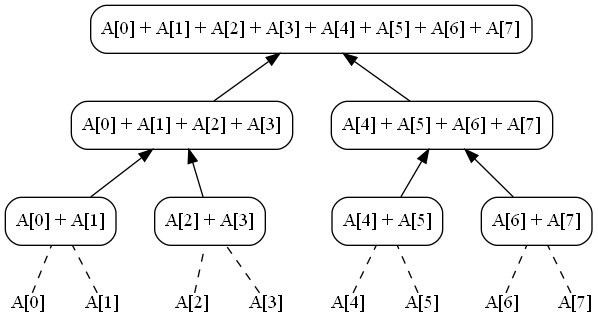
\includegraphics[width=1\textwidth]{divideconquer}
\end{minipage}
\caption{An example of \figref{fig:innerproductmpcvecdandc} for $n = 8$. 
Each level of tree is executed in parallel. This reduces the run time 
complexity from $O(n)$ to $O(log_{2}(n))$.}
\label{fig:treeexample}
\end{figure}

\figref{fig:innerproduct}, \figref{fig:innerproductmpc}, and \figref{fig:innerproductmpcvec} 
show a full transformation from high-level C-like source that computes the inner produce of 2 arrays {\sf A} and {\sf B}, 
to a fully vectorized MPC source that can be turned into an optimal MPC schedule. \figref{fig:treeexample}
shows a visualization of the execution performed for $n = 8$.
Initially in \figref{fig:innerproduct} and \figref{fig:innerproductmpc} $N$ 
multiplications and additions are performed. However in \figref{fig:innerproductmpcvec} 
the multiplications can be flattened to one operation, while the
additions are still performed sequentially with a \emph{for} loop. In  \figref{fig:innerproduct} the time
complexity of the algorithm is $O(n)$ where $n$ is the length of the array. Removing
the multiplication from the loop body does not reduce the asymptotic complexity, however,
in practice this has significant impact as in MPC multiplication is an expensive operation that
requires remote computation of the parties while addition is local and inexpensive. 
In addition, vectorization of multiplication allows for the addition operation to be isolated and 
additionally optimized, using divide-and-conquer techniques, which reduces the complexity to
$O(log_2(n))$ \cite{Farzan2017}. The transformation for inner product is shown in \figref{fig:innerproductmpcvecdandc}.

The great benefit of MPC amortizations is, due to the circuit representation, there is no inherent 
limit of the scale of parallelization. As we mentioned in \secref{sec:hpcparallelization} general
scheduling is a NP-Hard problem \cite{Cytron1984},\cite{Graham1971} however this is due to the restrictions
on the number of processors, with an unlimited number of processors the problem can be solved in polynomial time
\cite{Darte2000}. We claim that our problem is substantially different. In summary, the MPC amortization problem 
is different from the HPC parallelization problem because: in MPC we can assume unlimited bandwidth, and also 
we can only ``schedule in parallel'' two operations that are the same; in HPC we have a fixed number of processors, 
and we can schedule in parallel any two operations. Thus, we avoid some of the limitations that are present in HPC 
scheduling, while MPC imposes its own limitations and constraints. 


This leads to our two main problems. 

\begin{problem}
Given a loop body, find a schedule for the execution of statements in that body within a single iteration
of the loop taking into account intra-loop dependencies. This schedule should improve or not effect the
performance of the loop.
\label{problem:prob1}
\end{problem}

\begin{problem}
Given a loop, compute a schedule for the execution of the loop that takes into account intra-loop and across-loop dependencies.
\label{problem:prob2}
\end{problem}

Our work computes a schedule for a given a loop. A schedule is a sequence of MPC-primitives, as shown in~\figref{fig:muximpsyntax}.

%For the general case with arbitrary across-loop dependences, our vectorization may not be optimal.
%However, it is optimal under certain restrictions on across-loop dependences and certain assumptions about the loop body schedule. We elaborate 
%on these restrictions in \secref{sec:theoreticalguarentees}. Additionally in \secref{sec:results} we show that in practice, many of the 
%programs we saw from the HyCC benchmark did not violate these assumptions. %\ana{THIS MAY NEED TO CHANGE!!!} 
%\ana{Lindsey, check if this is true :) or we need to tone this down.} \lindsey{toned down!}

%\lindsey{not sure where to put this}
%\begin{itemize} 
%  \item Every dependency exists regardless of which iteration is being computed
%  \item Every dependency is remains unchanged regardless of which iteration is being computed
%\end{itemize} 



